\section{Background and previous work}

\subsection{Background}
\gls{vqa} models have drawn recent interest in the computer vision community as they allow text queries to question image content. This has given way to a number of novel applications in the space of model reasoning~\cite{wang2015explicit,cadene2019murel,wu2021multi,jing2022maintaining}, medical diagnosis~\cite{nguyen2019overcoming,vu2020question,gupta2021hierarchical,zhan2020medical} and counterfactual learning~\cite{agarwal2020towards,chen2020counterfactual,abbasnejad2020counterfactual}. With the ability to combine language and image information in a common model, it is unsurprising to see a growing use of \gls{vqa} methods.

Despite this recent progress, however, a number of important challenges remain when making \gls{vqa}s more proficient. For one, it remains extremely challenging to build \gls{vqa} datasets that are void of bias. Yet this is critical to ensure subsequent models are not learning spurious correlations or shortcuts~\cite{teney2020unshuffling}. This is particularly daunting in applications where domain knowledge plays an important role (\eg,  medicine~\cite{he2020pathvqa,lau2018dataset,do2021multiple}). Alternatively, ensuring that responses of a \gls{vqa} are coherent, or {\it consistent}, is paramount as well. That is, \gls{vqa} models that answer differently about similar content in a given image imply inconsistencies in how the model interprets the inputs. A number of recent methods have attempted to address this using logic-based approaches~\cite{gokhale2020vqa}, rephrashing~\cite{shah2019cycle}, question generation~\cite{ribeiro2019red,ray2019sunny, goel2021iq} and regularizing using consistency constraints~\cite{tascon2022consistency}. In this work, we follow this line of research and look to yield more reliable \gls{vqa} models.

\begin{figure}[!b]
\centering
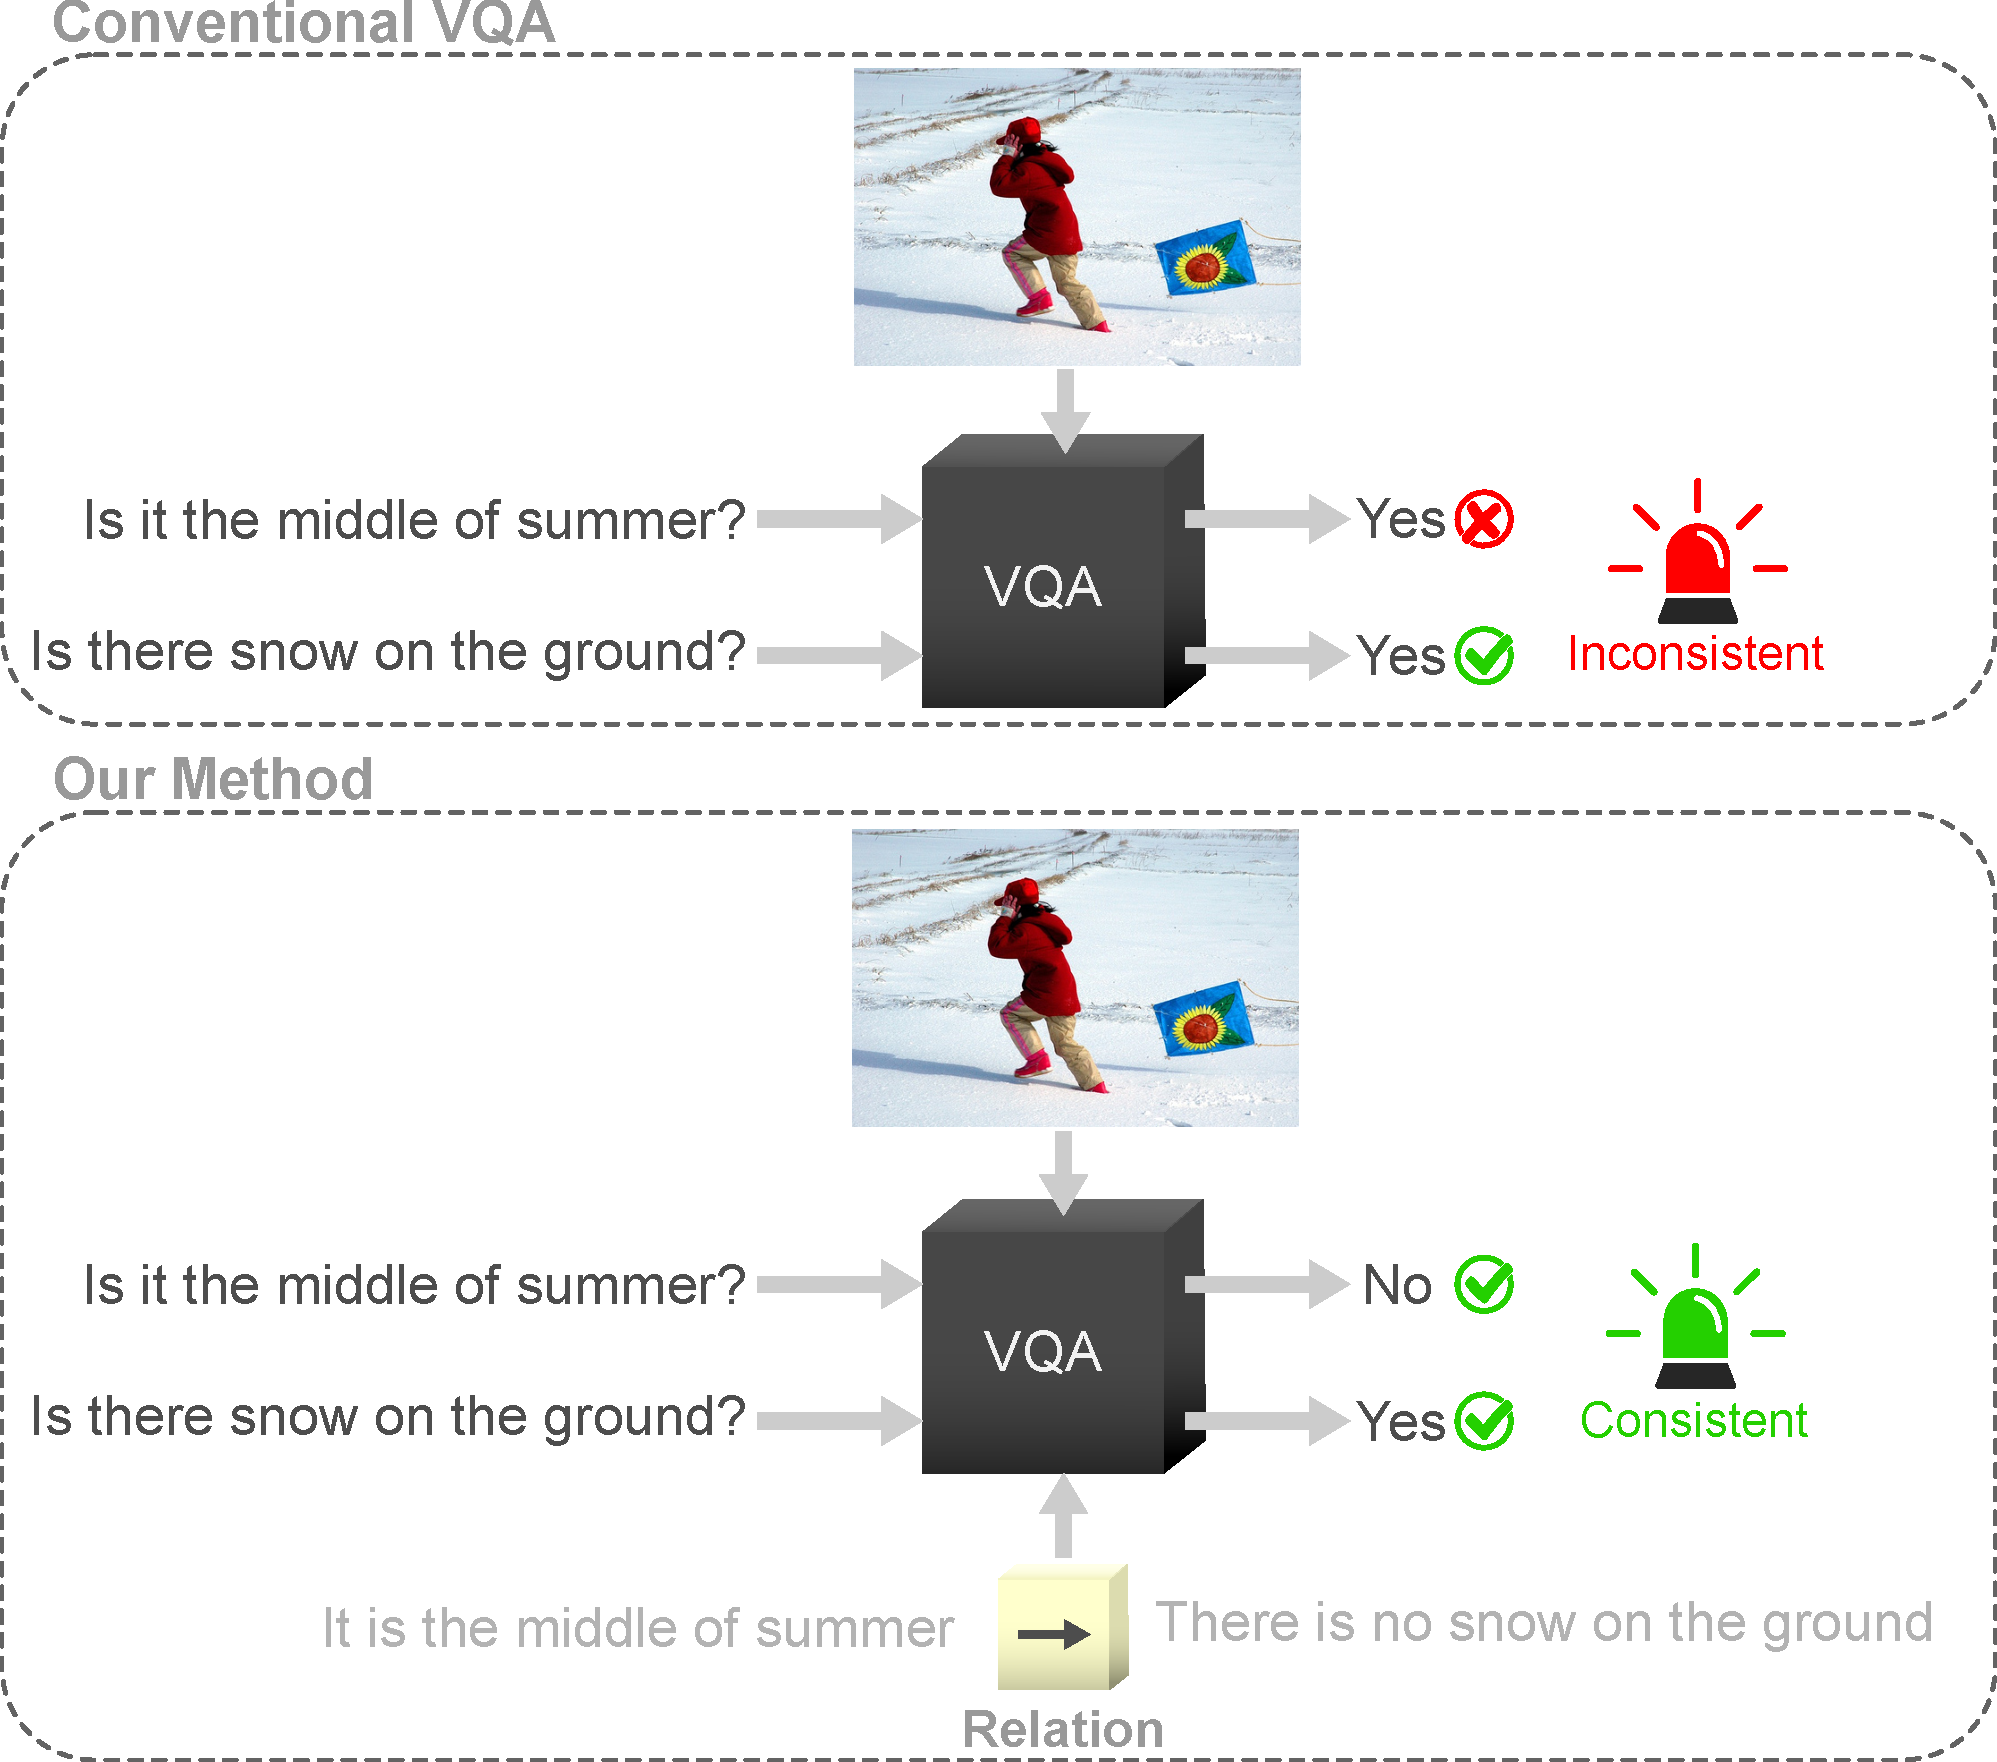
\includegraphics[width=0.6\textwidth]{Figures/Part2_Consist/02_logic/image_intro.pdf}
\caption{\textbf{Top:} Conventional VQA models tend to produce inconsistent answers as a consequence of not considering the relations between question and answer pairs. \textbf{Bottom:} Our method learns the logical relation between question and answer pairs to improve consistency.
} 
\label{fig:image_intro}
\end{figure}

We wish to ensure that \gls{vqa} models are consistent in answering questions about images. This implies that if multiple questions are asked about the same image, the model's answers should not contradict themselves. For instance, if one question about the image in \fig~\ref{fig:image_intro} asks ``Is there snow on the ground?", then the answer inferred should be consistent with that of the question ``Is it the middle of summer?" As noted in~\cite{selvaraju2020squinting}, such question pairs involve reasoning and perception, and consequentially lead the authors to define inconsistency when the reasoning and perception questions are answered correctly and incorrectly, respectively. Along this line,~\cite{tascon2022consistency} uses a similar definition of inconsistency to regularize a \gls{vqa} model meant to answer medical diagnosis questions that are hierarchical in nature. What is critical in both cases, however, is that the consistency of the \gls{vqa} model depends explicitly on its answers, as well as the question and true answer. This hinges on the assumption that perception questions are sufficient to answer reasoning questions. Yet, for any question pair, this may not be the case. As such, the current definition of consistency (or inconsistency) has been highly limited and does not truly reflect how \gls{vqa}s should behave. 

To address the need to have self-consistent \gls{vqa} models, we propose a novel training strategy that relies on logical relations. To do so, we re-frame question-answer (QA) pairs as propositions and consider the relational construct between pairs of propositions. This construct allows us to properly categorize pairs of propositions in terms of their logical relations. From this, we introduce a novel loss function that explicitly leverages the logical relations between pairs of questions and answers in order to enforce that \gls{vqa} models be self-consistent. However, datasets typically do not contain relational information about QA pairs, and collecting this would be extremely laborious and difficult. To overcome this, we propose to train a dedicated language model that infers logical relations between propositions.
Our experiments show that we can effectively infer logical relations from propositions and use them in our loss function to train \gls{vqa} models that improve state-of-the-art methods via consistency. We demonstrate this over two different \gls{vqa} datasets, against different consistency methods, and with different \gls{vqa} model architectures.

\subsection{Previous Work}
Since its initial presentation in Antol et al.~\cite{antol2015vqa}, \gls{vqa} has thoroughly advanced. Initial developments focused on multimodal fusion modules, which combine visual and text embeddings~\cite{nam2017dual,cadene2019murel}. From basic concatenation and summation~\cite{antol2015vqa} to more complex fusion mechanisms that benefit from projecting the embeddings to different spaces, numerous approaches have been proposed~\cite{fukui2016multimodal,kim2016hadamard,ben2017mutan}. The addition of attention mechanisms~\cite{kim2018bilinear, nam2017dual,cadene2019murel} and subsequently transformer architectures~\cite{vaswani2017attention} has also contributed to the creation of transformer-based \gls{vlm}, such as LXMERT, which have shown state-of-the-art performances~\cite{tan2019lxmert}. 

More recently, methods have proposed to improve other aspects of \gls{vqa}, including avoiding shortcut learning and biases~\cite{dancette2021beyond,han2021greedy}, improving 3D spatial reasoning~\cite{banerjee2021weakly}, Out-Of-Distribution (OOD) generalization~\cite{cao2021linguistically,teney2020unshuffling}, improving transformer-based vision-language models~\cite{yang2021auto,zhou2021trar}, external knowledge integration~\cite{ding2022mukea,gao2022transform} and model evaluation with visual and/or textual perturbations~\cite{gupta2022swapmix,walmer2022dual}. With the awareness of bias in \gls{vqa} training data, some works have also addressed building better datasets (\eg, VQAv2.0~\cite{goyal2017making}, VQA-CP~\cite{agrawal2018don}, CLEVR~\cite{johnson2017clevr} and GCP~\cite{hudson2019gqa}).

Furthermore, these developments have now given rise to \gls{vqa} methods in specific domains. For instance, the VizWiz challenge~\cite{gurari2018vizwiz,gurari2019vizwiz,chen2022grounding} aims at creating \gls{vqa} models that can help visually impaired persons with routine daily tasks, while there is a growing number of \gls{medvqa} works with direct medicine applications~\cite{nguyen2019overcoming,gupta2021hierarchical,vu2020question,zhan2020medical}. 

\subsubsection{Consistency in VQA} Consistency in \gls{vqa} can be defined as the ability of a model to produce answers that are not contradictory. This is, given a pair of questions about an image, the answers predicted by a \gls{vqa} model should not be contrary (\eg answering ``Yes" to ``Is it the middle of summer?" and ``Winter" to ``What season is it?"). Due to its significance in reasoning, consistency in \gls{vqa} has become a focus of study in recent years~\cite{ribeiro2019red,shah2019cycle,gokhale2020vqa,selvaraju2020squinting,jing2022maintaining}. Some of the first approaches for consistency enhancement focused on creating re-phrasings of questions, either by dataset design or at training time~\cite{shah2019cycle}. Along this line, entailed questions were proposed~\cite{ribeiro2019red,gokhale2020vqa}, such that a question generation module was integrated into a \gls{vqa} model~\cite{ray2019sunny,goel2021iq}, used as a benchmarking method to evaluate consistency~\cite{yuan2021perception} or as a rule-based data-augmentation technique~\cite{ribeiro2019red}. Other approaches tried to shape the embedding space by imposing constraints in the learned representations~\cite{teney2019incorporating} and by imposing similarities between the attention maps of pairs of questions~\cite{selvaraju2020squinting}. Another work~\cite{tascon2022consistency} assumed entailment relations between pairs of questions to regularize training. A more recent approach attempts to improve consistency by using graph neural networks to simulate a dialog in the learning process~\cite{jing2022maintaining}. 

While these approaches show benefits in some cases, they typically only consider that a subset of logical relationships exists between pairs of question-answers or assume that a single relation holds for all QA pairs. Though true in the case of re-phrasings, other question generation approaches cannot guarantee that the produced questions preserve unique relations or that grammatical structure remains valid. Consequently, these methods often rely on metrics that either over or under-estimate consistency by relying on these assumptions. In the present work, we propose a strategy to alleviate these limitations by considering all logical relations between pairs of questions and answers. 

\subsubsection{Entailment Prediction} \glsxtrfull{nli}, or \gls{rte}, is the task of predicting how two input sentences (namely \textit{premise} and \textit{hypothesis}) are related, according to three pre-established categories: entailment, contradiction and neutrality~\cite{maccartney2008modeling}. For example, if the premise is ``A soccer game with multiple males playing" and the hypothesis is ``Some men are playing a sport," then the predicted relation should be an entailment, because the hypothesis logically follows from the premise. Several benchmarking datasets (\eg, SNLI~\cite{young2014image}, MultiNLI~\cite{williams2017broad}, SuperGLUE~\cite{wang2019superglue}, WIKI-FACTCHECK~\cite{sathe2020automated} and ANLI~\cite{nie2019adversarial}) have contributed to the adaption of general-purpose transformer-based models like \gls{bert}~\cite{devlin2018bert}, RoBERTa~\cite{liu2019roberta} and DeBERTa~\cite{he2020deberta} for this task. In this work, we will leverage these recent developments to build a model capable of inferring relations between propositions.